\chapter{Grundlagen}
\label{ch:grund}
\rm

\section{Algorithmen}\label{sec:alg}
In diesem Kapitel sollen die Extraktionsalgorithmen vorgestellt werden, aus denen die im \textbf{Kapitel \ref{ch:optarm}} beschriebenen FeatureSets zusammengesetzt sind, die f�r die Laufzeitanalyse des Codes verwendet werden. Hierf�r werden diese in zwei Bereiche unterteilt, einmal die Features, welche im Zeitbereich arbeiten (\textbf{\ref{subsec:zeit}}) und diese die im Frequenzbereich arbeiten (\textbf{\ref{subsec:freq}}). Diese Unterteilung wurde aus \cite{haller2008} �bernommen.

\subsection{Notation von Ausdr�cken und Variablen}\label{subsec:note}

Hier sollen kurz die verwendeten Ausdr�cke und Variablen eingef�hrt werden, die f�r die sp�tere Definition der einzelnen Features ben�tig werden (\textbf{Tabelle \ref{tab:note}}), wie sie in  \cite{haller2008} und \cite{Theimer2008} definiert sind.

\begin{table*}[ht]
	\centering
		\begin{tabular}{p{6cm} | c}
			\textbf{Ausdruck} & \textbf{Formel}\\
			\hline
			\hline
			Anzahl der Zeitfenster im Musikst�ck & $L_{total}~=~\left\lceil \frac{N_{total}}{N} \right\rceil$ \\
			Anzahl der Frequenzwerte & $K$ \\
			Anzahl der Samples im Musikst�ck & $N_{total}$ \\
			Amplitude der Spektralkomponente & $A(k)~=~\left|X(k)\right|$ \\
			Amplitude der Spektralkomponente im Zeitfenster l & $A^{(l)},~l\in[1,L_{total}]$\\
			Diskrete Fouriertransformation & $X(k)~=~\sum\limits^{N-1}_{n=0}x(n)\cdot W^
			{kn}_N,~W_N~=~e^{-j\frac{2\pi}{N}},~K~=~N$\\
			diskrete Spektralkomponente & $X(k)$ \\
			diskretes Zeitsignal & $x(n),\ n\in[0,N_{total}~-~1]$\\
			Frequenzwert & $k\in[0,~K]$ \\
			L�nge eines Zeitfensters & $N$\\
			Samplingfrequenz in Hz & $f_{s}$
		\end{tabular}
	\caption{Tabelle der verwendeten Ausdr�cke und Variablen}
	\label{tab:note}
\end{table*}


\subsection{Features des Zeitbreichs}\label{subsec:zeit}

\subsubsection{Root Mean Square (RMS)}\label{subsubsec:rms}
Root Mean Square oder auch das quadratische Mittel normiert die einzelnen Signalenergien innerhalb eines Zeitfensters (\textbf{Formel \ref{eqn:rms}}).\cite{haller2008}\cite{Theimer2008}

\begin{equation}
	\label{eqn:rms}
	x_{rms}~=~\sqrt{\frac{1}{N}\sum^{N-1}_{n=0}x^{2}(n)}
\end{equation}

\subsubsection{Low Energy}\label{subsubsec:le}

Low Energy fasst meherere aufeinander folgende Zeitfenster $n$ zu einem sogenannten Analysezeitraum zusammen und gibt die Rate der Zeitfenster an, deren RMS unter dem Mittel aller RMS im Analysezeitraum liegen (\textbf{Formel \ref{eqn:le}}). Hierf�r sei $N_{a}$ die Anzahl der berachteten Zeitfenster im Analysezeitraum.\cite{haller2008}\cite{Theimer2008}

\begin{equation}
	\label{eqn:le}
	r_{low}~=~\frac{1}{N_{a}}\sum^{N_{a}-1}_{i=0}u(\mu_{rms}~-~x_{rms}(n))
\end{equation}
mit \[\mu_{rms}~=~\frac{1}{N_{a}}\sum^{N_{a}-1}_{i=0}x_{rms}(n)\] und \[u(x)~=~\left\{ \begin{array}{ll} 
1 & \textrm{f�r } x~>~0 \\
0 & \textrm{f�r } x~\leq~0\\
\end{array}\right.\]
 

\subsubsection{Zero Crossing Rate}\label{subsubsec:zcr}

Bei der Zero Crossing Rate werden die Auftreten von Vorzeichenwechseln innerhalb eines Zeitfensters berechnet. Diese Rate gibt ein Ma� f�r den hochfrequenten Anteil des Signals an (\textbf{Formel \ref{eqn:zero}}).\cite{haller2008}\cite{Theimer2008}

\begin{equation}
	\label{eqn:zero}			   r_{zcr}~=~\frac{1}{2(N~-~1)}\sum^{N-2}_{n=0}\left|sgn~x(n~+~1)~-~sgn~x(n)\right|
\end{equation}



\subsection{Features des Frequenzbereichs}\label{subsec:freq}

\subsubsection{Fast Fourier Transformation (FFT)}\label{subsubsec:fft}

Unter dem Begriff \textit{Fast Fourier Transformation} werden werden Algorithmen zusammengefasst, die eine schnelle und effiziente Berechnung von \textit{diskreten Fourier-Transformationen (DFT)} bieten. Diese effizienten Algorithmen kann man im wesentlichen in zwei Gruppen unterteilen, diejenigen die mit Zeitzerlegung (\textbf{\ref{ph:dit}}) und diejenigen die mit Frequenzzerlegung (\textbf{\ref{ph:dif}}) arbeiten.\\
F�r beide Gruppen von Algorithmen wird immer eine Operation ben�tigt, die entweder die Eing�nge oder die Ausg�nge in einer bestimmten Form sortiert. Diese Operation wird als \textit{Bitumkehrordnung} oder engl. \textit{bit-reversed order} bezeichnet (\textbf{\ref{ph:bit}}).\cite{Opp1999}

\paragraph{FFT mit Zeitzerlegung (DIT)}\label{ph:dit}$\;$ \\

\begin{figure}[ht]
	\centering
		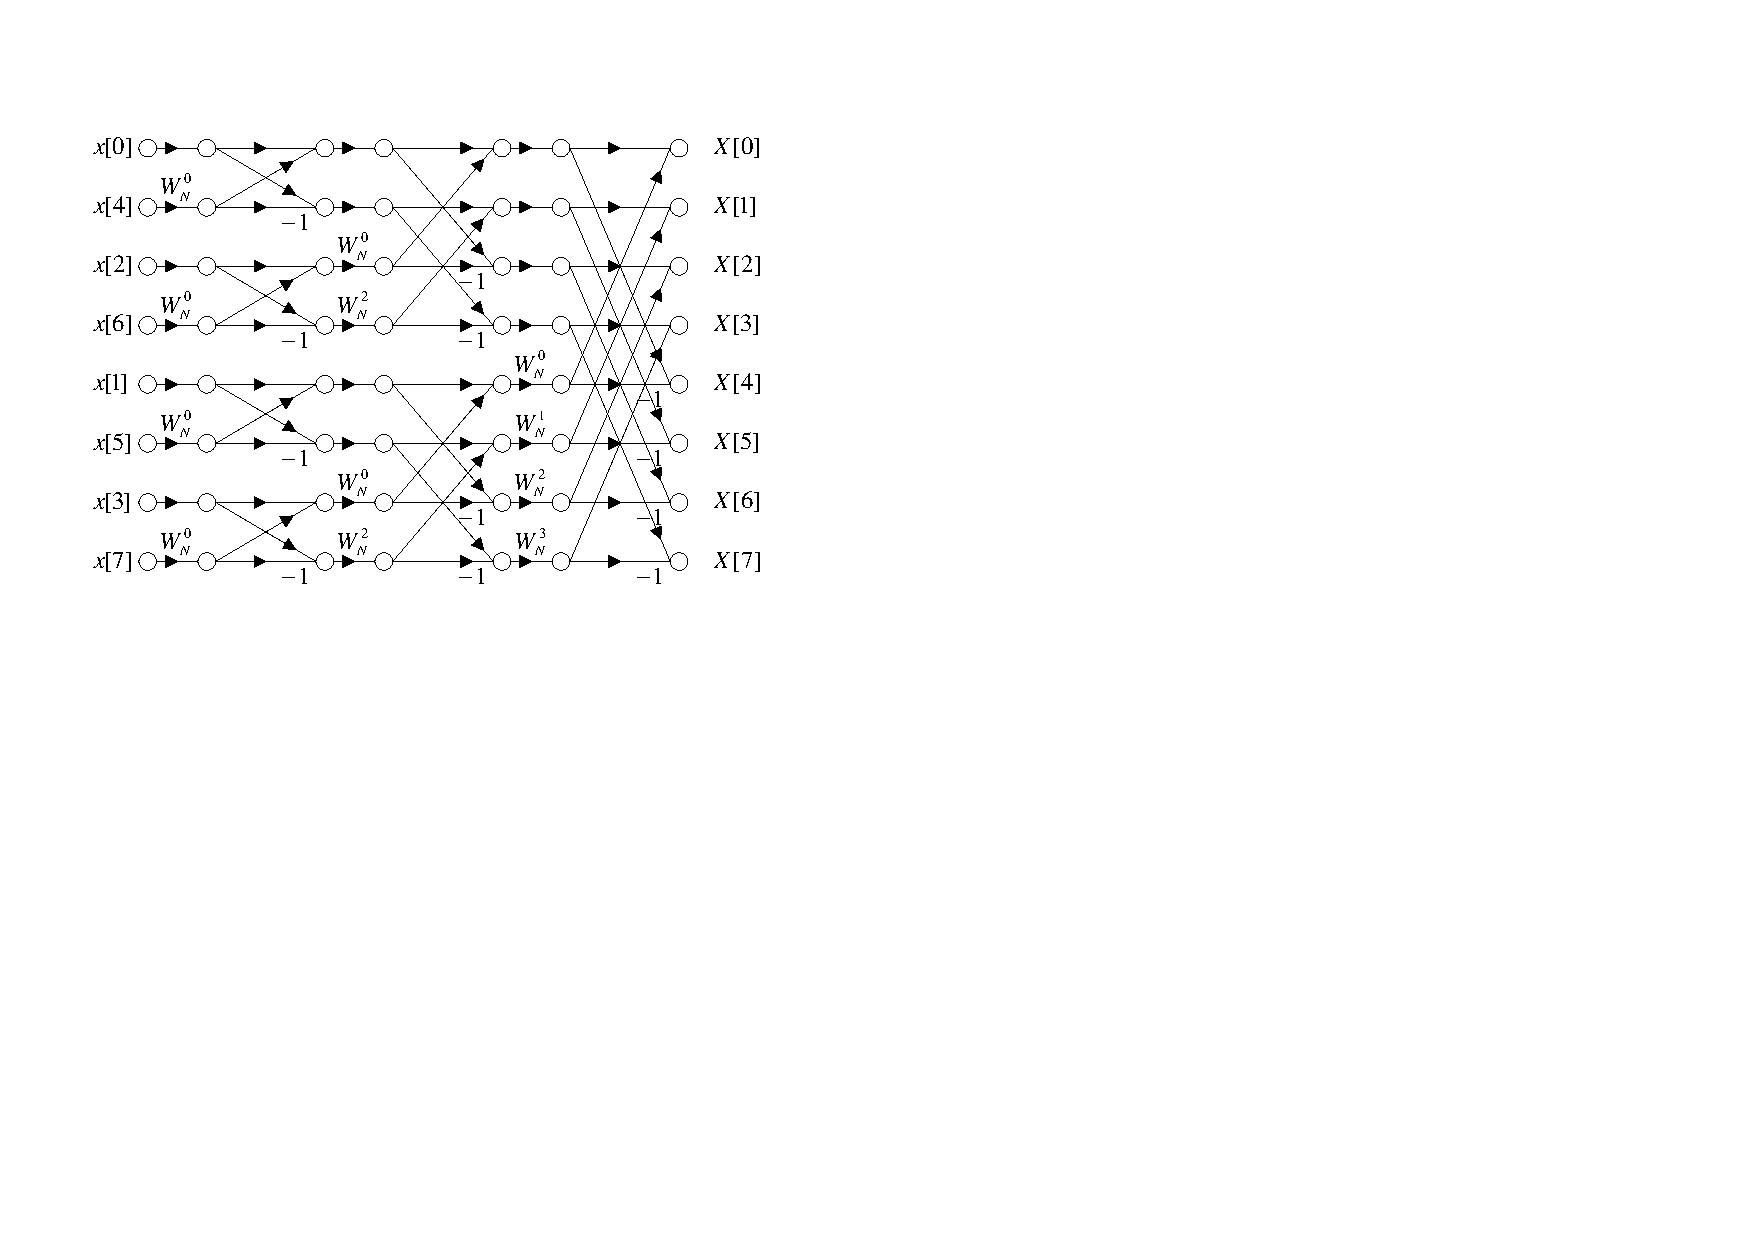
\includegraphics{../Pictures/DIT.pdf}
	\caption{Signalflu�graph einer 8-Punkte DFT mit Zeitzerlegung\cite{Opp1999}}
	\label{fig:dit}
\end{figure}

\paragraph{FFT mit Frequenzzerlegung (DIF)}\label{ph:dif}$\;$ \\

\begin{figure}[ht]
	\centering
		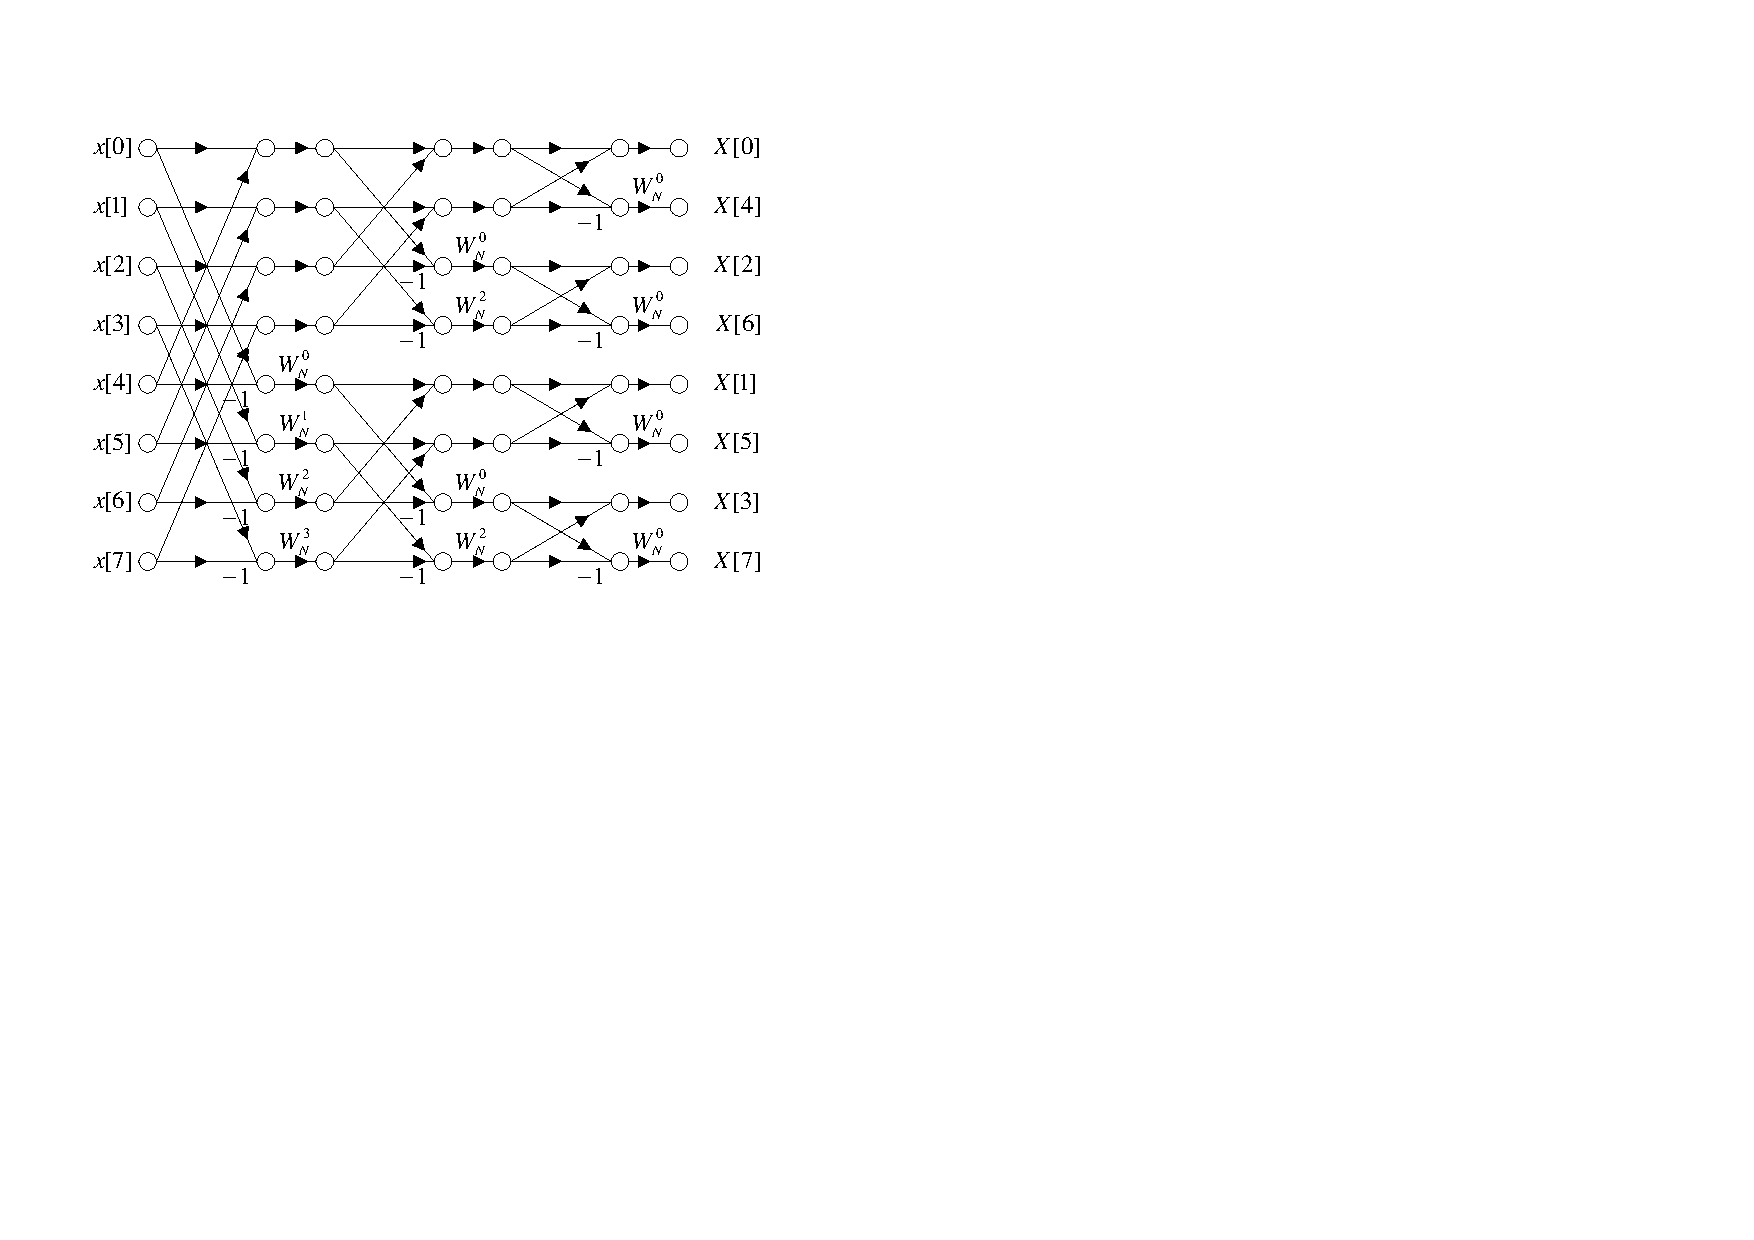
\includegraphics{../Pictures/DIF.pdf}
	\caption{Signalflu�graph einer 8-Punkte DFT mit Frequenzzerlegung\cite{Opp1999}}
	\label{fig:dif}
\end{figure}

\paragraph{Bitumkehrungordnung (bit-reversed order)}\label{ph:bit}$\;$ \\

Wie man in \textbf{Abbildung \ref{fig:dit}} und \textbf{Abbildung \ref{fig:dif}} gut erkennen kann, liegen entweder die Eing�nge oder die Ausg�nge in einer nicht numerisch sortierten Form vor. Diese Sortierung ergibt sich aus den in (\textbf{\ref{ph:dit}}) und (\textbf{\ref{ph:dif}}) gezeigten Algorithmen, diese folgt aber immer dem selben Schema.\\ 
Es werden die Indizes des Ein- oder Ausgangs anhand ihrer Bits vom \textit{Least Significant Bit (LSB)} zum \textit{Most Significant Bit (MSB)} sortiert, so dass pro Ebene in der oberen H�fte die Indizes stehen, die beim momentan betrachteten Bit eine 0 aufweisen.\\
Dieses Prinzip soll in \textbf{Tabelle \ref{tab:bit}} f�r 8-Bit lange Indizes veranschaulicht werden.

\begin{table}[ht]
	\centering
		\begin{tabular}{c | c | c | c}
			Position (dezimal) & Position (bin�r) & "`bit reversal"' (bin�r) & "`bit reversal"' (dezimal) \\
			\hline\hline
			0 & 000 & 000 & 0\\
			1 & 001 & 100 & 4\\
			2 & 010 & 010 & 2\\
			3 & 011 & 110 & 6\\
			4 & 100 & 001 & 1\\
			5 & 101 & 101 & 5\\
			6 & 110 & 011 & 3\\
			7 &	111 &	111 &	7
		\end{tabular}
	\caption{Bitumkehrordnung f�r 8-Bit Indizes\cite{haller2008}}
	\label{tab:bit}
\end{table}

\subsubsection{Chroma Vektor}\label{subsubsec:cv}

Der Chroma Vektor fasst alle Spektralkomponenten einer Tonh�he zusammen und fasst alle Frequenzen zu einer Oktave zusammen. Hierbei werden alle spektralen Amplituden des gleichen Halb- oder Vierteltons aufsummiert (\textbf{Formel \ref{eqn:cv}}).

\begin{equation}
	\label{eqn:cv}			   
	A_{chroma}\left(\widetilde{k}\right)~=~\sum_{k:~p(k)=\widetilde{k}} A(k)
\end{equation}

Z.B. f�r Viertelt�ne gilt

\[p(k)~=~\left\lfloor 24~log_{2}\left(\frac{2k}{N}\frac{f_{s}}{f_{1}}\right) \right\rfloor~mod~24\textrm{ und }f_{1}~=~440~Hz \]

F�r Halbt�ne m�sste 24 durch 12 ersetzt werden.\cite{haller2008}\cite{Theimer2008}

\subsubsection{Amplitude Of Maximum In Chromagram}\label{subsubsec:aomic}

Die maximale Amplitude des Chromagrams gibt den maximalen Chroma Vektor an und stellt daher die St�rke eines Tons in verschiedenen Oktavstufen dar (\textbf{Formel \ref{eqn:aomic}}).\cite{haller2008}\cite{Theimer2008}

\begin{equation}
	\label{eqn:aomic}			   
	A_{maxchroma}~=~\max_{\widetilde{k}}~A_{chroma}\left(\widetilde{k}\right)
\end{equation}

\subsubsection{Mel Frequency Cepstral Coefficients (MFCC)}\label{subsubsec:mfcc}

\subsubsection{Normalized Audio Spectrum Envelope}\label{subsubsec:nase}

\subsubsection{Octave Spectral Contrast}\label{subsubsec:osc}

Beim Octave Spectral Contrast wird das Frequenzspektrum als erstes via Bandpass-Filtern in Unterb�nder aufgeteilt (siehe \textbf{Tabelle \ref{tab:osc}}), danach werden f�r jedes Unterband \textit{spektrale Peaks} (\textbf{Formel \ref{eqn:peak}}) und\textit{spektrale Valleys}(\textbf{Formel \ref{eqn:valley}}) berechnet, wobei Peaks den harmonischen Komponenten und Valleys nicht-harmonischen Komponenten oder Rauschen des Unterbandes $b$ entsprechen. Hierbei werden die Power Spektren $P_{b,n}$ vorher so sortiert, dass $P_{b,1}\geq P_{b,2}\geq ... \geq P_{b,n}$ gilt. 

\begin{table}[ht]
	\centering
		\begin{tabular}{c | c}
			Filternummer & Frequenzbereich (Hz)\\
			\hline\hline
			0 & [0,0]\\
			1 & (0,100]\\
			2 & (100, 200]\\
			3 & (200, 400]\\
			4 & (400, 800]\\
			5 & (800, 1600]\\
			6 & (1600, 3200]\\
			7 & (3200, 6400]\\
			8 & (6400, 12800]\\
			9 & (12800, 22050]\\
			
		\end{tabular}
	\caption{Frequenzbereiche der Bandpass-Filter bei 44.1 kHz Sapmingfrequenz\cite{Lee2009}}
	\label{tab:osc}
\end{table}

\begin{equation}
	\label{eqn:peak}			   	
	Peak(b)~=~\log\left(\frac{1}{\alpha N_b}\sum\limits^{\alpha N_b}_{i=1}P_{b,i}\right)
\end{equation}
\begin{equation}
	\label{eqn:valley}			   	
	Valley(b)~=~\log\left(\frac{1}{\alpha N_b}\sum\limits^{\alpha N_b}_{i=1}P_{b,N_b - i+1}\right)
\end{equation}
Hierbei ist $\alpha$ ein Nachbarschaftsfactor, der in der Literatur mit 0,2 angenommen wird. Der spektrale Kontrast eines Unterbandes errechnet sich nun als Differenz von $Peak(b)$ und $Valley(b)$ (\textbf{Formel \ref{eqn:oscsc}}).
\begin{equation}
	\label{eqn:oscsc}			   	
	SC(b)~=~Peak(b)~-~Valley(b)
\end{equation}
Und der resultierende Featurevektor $x_{OSC}$ abschlie�end aus den Valleys und spektralen Kontrasten eines Auioframes (\textbf{Formel \ref{eqn:osc}}).\cite{Lee2009}

\begin{equation}
	\label{eqn:osc}			   	
	x_{OSC} = \left[Valley(0=,...,Valley(B-1),SC(0),...SC(B-1)\right]^T
\end{equation}

\subsubsection{Power Spectrum}\label{subsubsec:ps}

Das Power Spectrum berechnet sich indem man den Logarithmus des Amplitudenspektrums berechnet (\textbf{Formel \ref{eqn:ps}}).\cite{haller2008}

\begin{equation}
	\label{eqn:ps}			   	
	S(k)~=~10\cdot\log\limits_{10}\left(\frac{1}{N}A^2(k)\right)
\end{equation}



\subsubsection{Spectral Centroid}\label{subsubsec:sc}

Der Spectral Centroid gibt den Schwerpunkt des Amplitudenspektrums des Signals an (\textbf{Formel \ref{eqn:sc}}).\cite{haller2008}\cite{Theimer2008}

\begin{equation}
	\label{eqn:sc}			   	S_{centroid}~=~\frac{\sum\limits^{\frac{K}{2}-1}_{k=0}k~A(k)}{\sum\limits^{\frac{K}{2}-1}_{k=0}A(k)} 
\end{equation}

\subsubsection{Spectral Crest Factor}\label{subsubsec:scf}

Der Spectral Crest Factor stellt ein Ma� der spectralen Flachheit eines Frequenzbandes dar und ist im Wertebereich $\left[1,\infty\right]$ definiert. Hierbei bedeutet 1, dass alle spectral Ampilituden gleich sind und $\infty$ das garkeine Flachheit existiert (\textbf{Formel \ref{eqn:scf}}).\\
Dieser Factor wird auf folgenden Frequenzb�ndern berechnet:
\begin{itemize}
	\item 250 - 500 Hz ($k_{1l}$ - $K_{1u}$)
	\item 500 - 1000 Hz ($k_{2l}$ - $K_{2u}$)
	\item 1000 - 2000 Hz ($k_{3l}$ - $K_{3u}$)
	\item 2000 - 4000 Hz ($k_{4l}$ - $K_{4u}$)
\end{itemize}
\cite{Theimer2008}

\begin{equation}
	\label{eqn:scf}			   
	S_{crest}~=~frac{\max\limits_{k\in\left[k_{il},k_{iu}\right]}A(k)}{\frac{1}{k_{iu}~-~k_{il}~+~1}\sum\limits^{k_{iu}}_{k=k_{il}}A(k)}
\end{equation}

\subsubsection{Spectral Flux}\label{subsubsec:sf}

Der Spectral Flux ist definiert als die quadrierte Differenz zwischen den normalisierten Betragsspektren von zwei aufeinander folgenden Zeitfenstern (\textbf{Formel \ref{eqn:sf}}).\cite{haller2008}\cite{Theimer2008}

\begin{equation}
	\label{eqn:sf}			   
	S_{flux}~=~\frac{2}{K}\sum\limits^{\frac{K}{2}-1}_{k=0}\left( A^{(l)}(k)~-~A^{(l-1)}(k)\right)^2
\end{equation}


\subsubsection{Spectral Rolloff}\label{subsubsec:sr}

Als Spectral Rolloff bezeichnet man der Frequenzwert ($k_{rolloff}$) unter dem sich eine bestimmte Prozentzahl ($p_{rolloff}$) der Spektralwerte konzentrieren (\textbf{Formel \ref{eqn:sr}}). \cite{haller2008}\cite{Tza2002}

\begin{equation}
	\label{eqn:sr}			   
	\sum^{k_{rolloff}}_{k=0}A(k)~=~p_{rolloff}~\cdot~\sum^{\frac{K}{2}-1}_{k=0}A(k)
\end{equation}

\subsubsection{Sub-Band Energy Ratio}\label{subsubsec:sber}

Die Sub-Band Energy Ratio gibt die Verteilung der Spektralenergy auf die Frequenzintervalle $\left[0,\frac{f_s}{16}\right)$,$\left[\frac{f_s}{16},\frac{f_s}{8}\right)$,$\left[\frac{f_s}{8},\frac{f_s}{4}\right)$ und $\left[\frac{f_s}{4},\frac{f_s}{2}\right)$ an und kann in Indexbereiche $\left[0,\frac{K}{16}\right)$,$\left[\frac{K}{16},\frac{K}{8}\right)$,$\left[\frac{K}{8},\frac{K}{4}\right)$ und $\left[\frac{K}{4},\frac{K}{2}\right)$ �berf�hrt werden (\textbf{Formel \ref{eqn:sber}}).\cite{Theimer2008}

\begin{equation}
	\label{eqn:sber}			   
	S_1~=~\frac{\sum\limits^{\frac{K}{16}-1}_{k=0}A^2(k)}{\sum\limits^{\frac{K}{2}-1}_{k=0}A^2(k)},~S_2~=~\frac{\sum\limits^{\frac{K}{8}-1}_{k=\frac{K}{16}}A^2(k)}{\sum\limits^{\frac{K}{2}-1}_{k=0}A^2(k)},S_3~=~\frac{\sum\limits^{\frac{K}{0}-1}_{k=\frac{K}{8}}A^2(k)}{\sum\limits^{\frac{K}{2}-1}_{k=0}A^2(k)},S_1~=~\frac{\sum\limits^{\frac{K}{2}-1}_{k=\frac{K}{4}}A^2(k)}{\sum\limits^{\frac{K}{2}-1}_{k=0}A^2(k)}
\end{equation}


\section{Profiling}\label{sec:prof}
Der Begriff Profiling bescheibt Methoden, mit denen das Verhalten von Applikationen auf Systemebene analysiert werden k�nnen, hierzu z�hlen Analysen der Laufzeit, der Schreib- und Lesezugriffe und auch die Verh�ltnisse von Instuktionen und Takten zueinander. Im Folgenden werden nun Beispielhaft die Profilingmethoden der Laufzeitmessung, der richtigen Vorhersagen des Vorladens in den Cache (sog. Cache Hits), sowie die Betrachtungen des Verh�ltnisses von Takt und Instuktionen (Instructions per Cycle (IPC) und Cycle per Instruction (CPI)).

\subsection{Laufzeitanalyse}\label{subsec:time}

\subsection{Cache Hits}\label{subsec:cache}

\subsection{IPC und CPI}\label{subsec:ipccpi}

